\chapter{Challenge II}
\section{Outline}
\begin{enumerate}
   \item Each subject manages a list with its own capabilities
   
   \item The operation field of a capability is encrypted with a key private to the security kernel SK
   
   \item To request operation Op on object O, a subject S sends to SK a message with S, O, Op and the encrypted capability
   
   \item SK decrypts the capability and, if it enables Op on O, it asks O to create a channel with S to execute OP
   
   \item O destroys the channel when Op ends
\end{enumerate}

\begin{figure}[htbp]
   \centering
   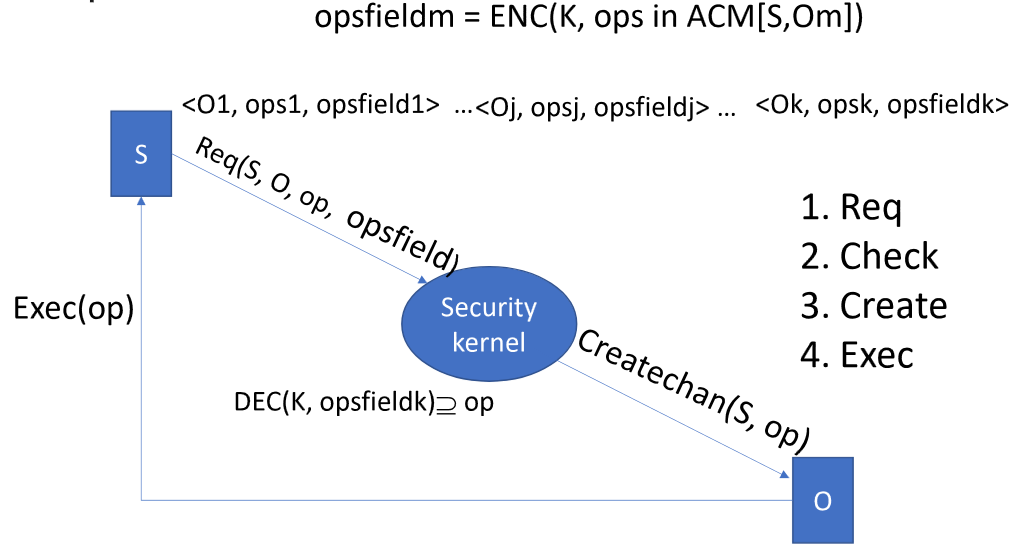
\includegraphics{images/challenge_2.png}
   \caption{Protocol schema}
   \label{fig:challenge_2}
\end{figure}

\subsection{Request}
Discover vulnerabilities in the proposed protocol or in the overall system under the assumption that there are no vulnerabilities in the encryption algorithm,
i.e. K cannnot be discovered because of  mathematical vulnerabilities.

\section{Proposed Solutions}
Below are listed possible vulnerabilities with some form of categorization,
although they may be related and/or not mutually exclusive.

\note{
   Despite the challenge title being \textit{"Capture-the-Flag"},
   the following vulnerabilities are {--}briefly{--} discussed and addressed from a "security" point of view,
   however they may be exploited as foundation to define and implement CTF competitions.
}

\subsection{Vulnerability 1 - Authentication}

First of all we can observe that the lack of \textbf{authentication} allows an attacker to impersonate the \texttt{Security Kernel},
and thus to invoke \texttt{Createchan(S,op)} on objects, choosing arbitrarily \texttt{S} and \texttt{op} and the destination object.

% Besides, the attacker (\textit{subject} \texttt{A}), assuming he doesn't own a capability \texttt{C}, but owns a secret,
% may change the subject field in \texttt{Req(S,O,op,opsfield)},
% writing \texttt{S'} (subject who owns the desired capability \texttt{C}) 

\subsection{Vulnerability 2 - Integrity}
The attacker, by posing theirself inbetween entities {---}implementing a \textit{man-in-the-middle} attack{---},
may manipulate any field on any sent message,
with the exception of \texttt{opsfield}, since he cannot discover the secret \texttt{K}.

In this way he may achieve \textit{Denial-of-Service} or may obtain capabilities he does not own.
\nl

\begin{center}
   \textit{"Each subject manages a list with its own capabilities"}.
\end{center}
Capabilities are usually stored in the subject,
but if it's not the case (e.g. distributed systems), depending on where and how such capabilities are stored and managed,
an attacker may manipulate them.

\subsection{Vulnerability 3 - Replay/Redirecting}

The attacker may sniff and record valid \texttt{Createchan(S,op)} and \texttt{Exec(op)} messages and replay them when desired.
Even if more costful and complex he may \textit{redirect}\footnote{equivalent to recording a message, dropping it, and replay it towards a different entity} them,
both obtaining access rights and denying the service for legitimate clients.

He may even copy \texttt{op} and \texttt{opsfield} and insert them in a \texttt{Req} sent by him.

\subsection{Bonus Vulnerabilities}
The following paragraphs do not refer to proper vulnerabilities,
but more generally to some security aspects  {---} or to vulnerabilities which are not as crucial/straightforward as the first ones{---}, which may result in undesired behaviour, possible intrusions, or simply bad system design choices.

\subsubsection{Vulnerability 4 - Overflow}
Probably not of interest here,
but every entity may be flooded by requests and messages,
resulting in a denial of service.

\subsubsection{Vulternability 5 - Lack of logging}
The protocol doesn't explicitly log anything,
which instead might be useful to track both legitimate and unlegitimate operation,
aiming to discover possible intrusion or to prove in a court of law that an intrusion has taken place.

\subsubsection{Vulnerability 6 - Encryption Info Leakage}
The problem outline states that \texttt{K} cannot be discovered due to mathematical vulnerabilities,
so we can leave aside all encryption attacks, mathematical vulnerabilities, etc.

However there are some techniques to infer information starting from the observation of one or multiple encrypted payloads,
exploiting statistical properties like size, entropy, and possibly others;
the attacker may also infer how costful (hence get an idea of which encryption method is being used) is to encrypt/decrypt fields by observing how much latency is introduced by communications which involve an encrypted payload.

\subsubsection{Vulnerability 7 - Least privilege violation}

The \textit{least privilege principle} states that a subject should own only the rights he needs to execute the operation he is currently performing.\\
The described protocol doesn't forbid a subject from requesting multiple operations on the same object before the previous ones have terminated,
resulting in multiple channels simulateneously open between an object \texttt{O} and a subject \texttt{S}, 
and in multiple rights owned by \texttt{S}.\\
This may be the desired outcome in some situations,
otherwise it results in the violation of the \textit{least privilege principle} and might be harmful.